\documentclass[12pt]{article}
\usepackage[margin=3cm]{geometry}
\usepackage{graphicx}
\usepackage{float}
\usepackage{url}
\usepackage{listings}
\usepackage{color}

\definecolor{mygreen}{rgb}{0,0.6,0}
\definecolor{mygray}{rgb}{0.5,0.5,0.5}
\definecolor{mymauve}{rgb}{0.58,0,0.82}
\lstset{ %
	xleftmargin=10em,
	backgroundcolor=\color{white},   % choose the background color; you must add \usepackage{color} or \usepackage{xcolor}
	basicstyle=\small,%\footnotesize,        % the size of the fonts that are used for the code
	breakatwhitespace=false,         % sets if automatic breaks should only happen at whitespace
	breaklines=false,                 % sets automatic line breaking
	captionpos=b,                    % sets the caption-position to bottom
	commentstyle=\color{mygreen},    % comment style
	deletekeywords={...},            % if you want to delete keywords from the given language
	escapeinside={\%*}{*)},          % if you want to add LaTeX within your code
	extendedchars=true,              % lets you use non-ASCII characters; for 8-bits encodings only, does not work with UTF-8
	%	frame=single,                    % adds a frame around the code
	keepspaces=true,                 % keeps spaces in text, useful for keeping indentation of code (possibly needs columns=flexible)
	keywordstyle=\color{blue},       % keyword style
	language=C, % the language of the code
	morekeywords={*,...},            % if you want to add more keywords to the set
	numbers=left,                    % where to put the line-numbers; possible values are (none, left, right)
	numbersep=5pt,                   % how far the line-numbers are from the code
	numberstyle=\small\color{mygray}, % the style that is used for the line-numbers
	rulecolor=\color{black},         % if not set, the frame-color may be changed on line-breaks within not-black text (e.g. comments (green here))
	showspaces=false,                % show spaces everywhere adding particular underscores; it overrides 'showstringspaces'
	showstringspaces=false,          % underline spaces within strings only
	showtabs=false,                  % show tabs within strings adding particular underscores
	stepnumber=1,                    % step between two line-numbers. If it's 1, each line will be numbered
	stringstyle=\color{mymauve},     % string literal style
	tabsize=2                  % sets default tabsize to 2 spac                  % show the filename of files included with \lstinputlisting; also try caption instead of title
}

\begin{document}

\begin{titlepage}
	\begin{center}
		
		
		% Upper part of the page. The '~' is needed because \\
		% only works if a paragraph has started.
		\vfill
		
		\textsc{\LARGE Lab 9: Standard Cell Based ASIC Design Flow}\\[1.5cm]
		
		\Large Adam Sumner\\[0.5cm]
		
		\Large Illinois Institute of Technology\\[0.5cm]
		
		\Large ECE 429-01\\[0.5cm]	
		
		\noindent
		\vfill
		\large \textbf{Lab Date:} November 9\textsuperscript{th}, 2015\hfill
		\large \textbf{Due Date:} November 18\textsuperscript{th}, 2015
		% Bottom of the page
	
		
	\end{center}
\end{titlepage}

\section{Introduction}
The purpose of this lab is to introduce the student to the concept of standard cell based ASIC design flow. The student will follow a tutorial to create the layout of an accumulator and then verify its correctness using equivalence checking.
\section{Theory/Pre-Lab}
\subsection{Theory}
Standard cell based ASIC design flow automatically synthesizes a chip layout from a register transfer level (RTL) description of a chip. The design flow utilizes the standard cell library to synthesize a chip layout according to design constraints including cost, performance, power consumption, etc. While this may seem like a nice tool to completely replace manual chip design, in practice, the tool will seldom generate a satisfactory design in the beginning. It is necessary for chip designers to understand the various steps of the design flow to guide the tool through multiple iterations before an optimum solution is found. In general, the standard cell based ASIC design flow consists of two steps: Logic Synthesis and Physical Design.
\subsubsection{Standard Cell Library}
A standard cell is a logic gate with a layout designed for a specific fabrication process. Standard cells for different types of logic gates and different sizes of the same gate are generally grouped into a standard cell library. Cells from the same library are most likely with the same height. Since the layout of a standard cell is known, characteristics of the cell can easily be obtained via SPICE simulations.
\subsubsection{Logic Synthesis}
The purpose of logic synthesis is to transform RTL descriptions of chip functionality into a netlist consisting of standard cells. Currently, it is very common to have datapath or arithmetic operations in a RTL description. The logic synthesis tool should first implement these operations as boolean logic. After this synthesis, the tool performs generic logic optimizations  on the design without any information form the standard cell library. After this, the netlist is generated with standard cells that have the same boolean functionality as the one generated by the tool in the beginning.
\subsubsection{Physical Design}
The purpose of the physical design is to create a physical implementation of the netlist consisting of standard cells. Due to the fact that every standard cell consumes silicon surface to form transistors, no two cell should overlap. Therefore, the most straightforward method is to place cells row by row, using metal layers to route wires.


\subsection{Pre-Lab}
The pre-lab involved familiarizing with Tutorial IV and the verilog code and testbench for the 8-bit accumulator. This was all done successfully.

\section{Implementation}
\subsection{Schematics}
\begin{figure}[H]
\centering
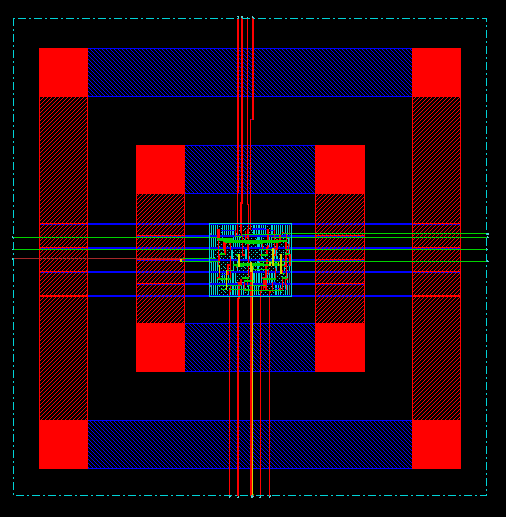
\includegraphics[width=1\linewidth]{layout-1}
\caption{Generated Layout Overview}
\label{fig:layout-1}
\end{figure}

\begin{figure}[H]
\centering
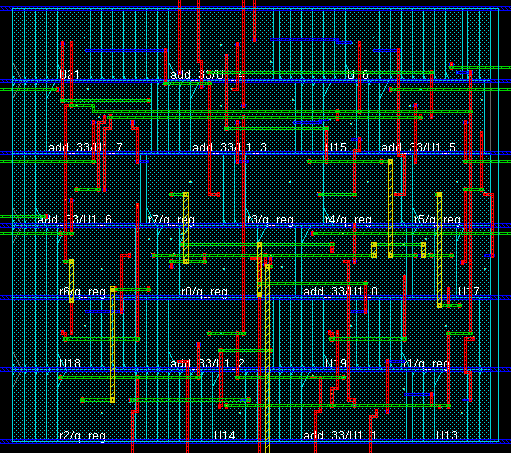
\includegraphics[width=1\linewidth]{layou-2}
\caption{Generated Layout Closeup}
\label{fig:layou-2}
\end{figure}

\begin{figure}[H]
\centering
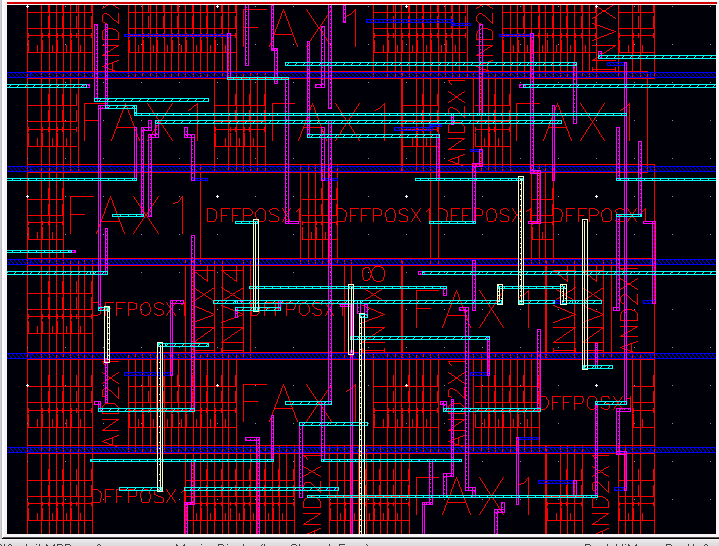
\includegraphics[width=1\linewidth]{layout-3}
\caption{Generated Layout Closeup 2}
\label{fig:layout-3}
\end{figure}

\begin{figure}[H]
\centering
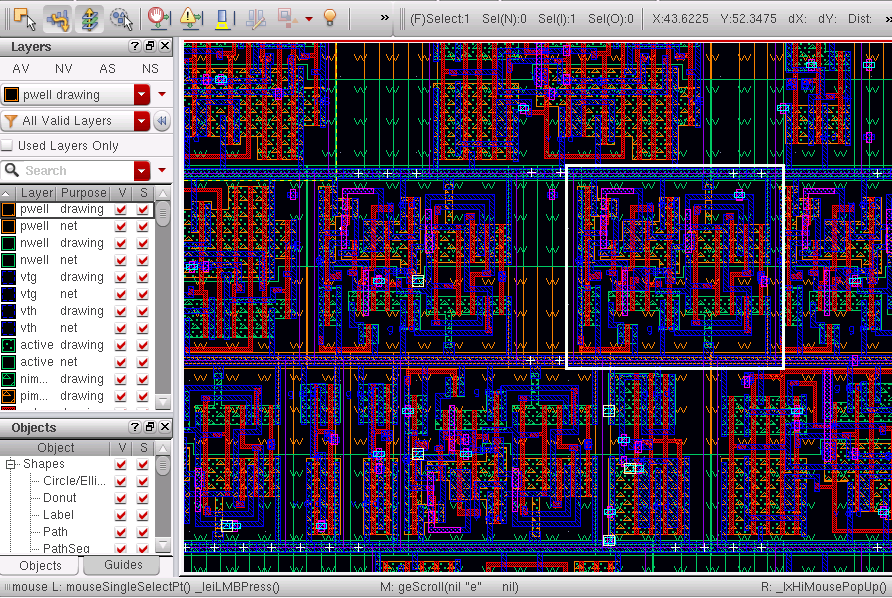
\includegraphics[width=1\linewidth]{layout-4}
\caption{Detailed Layout}
\label{fig:layout-4}
\end{figure}


\subsection{Procedure}
This lab involved following the instructions in Tutorial IV. This entailed checking verilog files for equivalence, generating a layout of the design, and then checking the layout for equivalence using Formality.

\subsection{Results}

\begin{figure}[H]
\centering
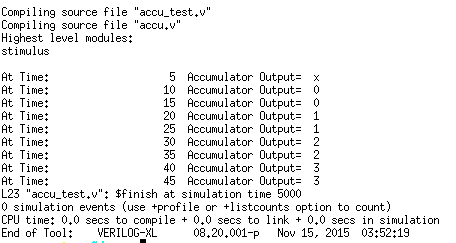
\includegraphics[width=0.5\linewidth]{verilog}
\caption{Initial Verilog Verfication}
\label{fig:verilog}
\end{figure}

\begin{figure}[H]
\centering
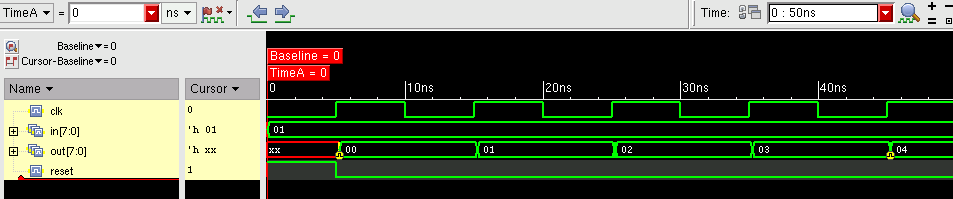
\includegraphics[width=1\linewidth]{waveform-intial}
\caption{Initial Waveform Verification of Verilog}
\label{fig:waveform-intial}
\end{figure}

\begin{figure}[H]
\centering
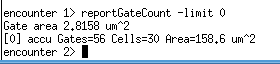
\includegraphics[width=0.5\linewidth]{area-report}
\caption{Area Report}
\label{fig:area-report}
\end{figure}

\begin{figure}[H]
\centering
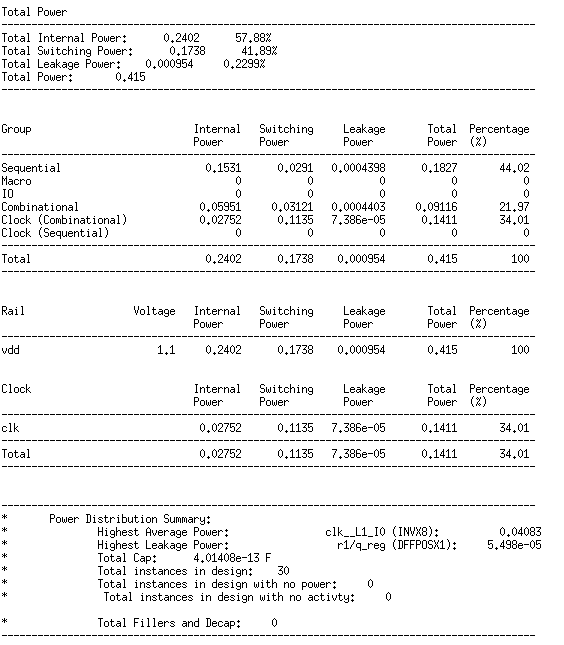
\includegraphics[width=0.7\linewidth]{power-report}
\caption{Power Report}
\label{fig:power-report}
\end{figure}

\begin{figure}[H]
\centering
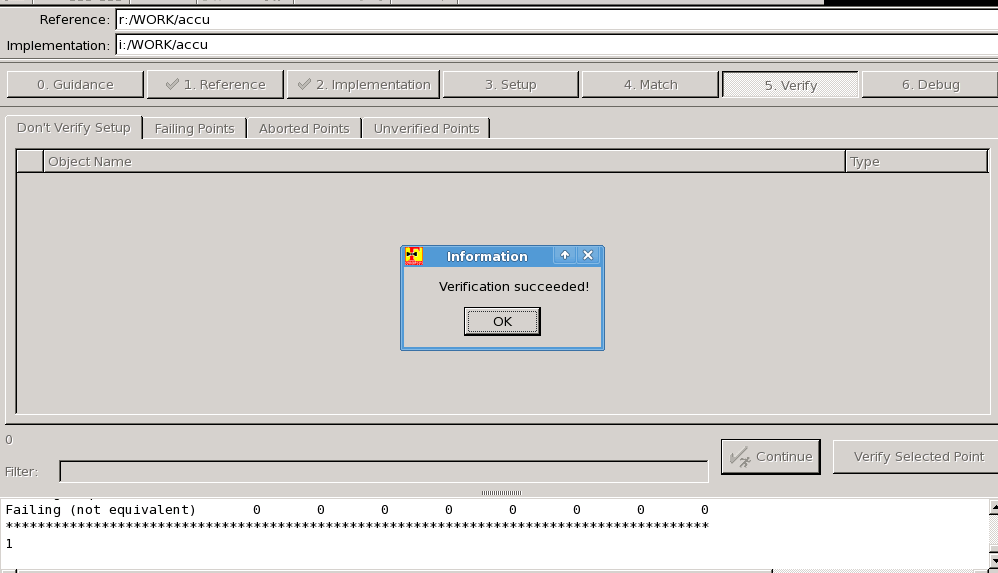
\includegraphics[width=0.7\linewidth]{fm-verification}
\caption{Formality Verification}
\label{fig:fm-verification}
\end{figure}

\subsection{Discussion}
Figures \ref{fig:layout-1}-\ref{fig:layout-4} show the generated layout design from the accumulator verilog file. From the results gathered in Figures \ref{fig:verilog}-\ref{fig:fm-verification}, it is clear that the layout was successfully generated and has equivalent functionality to the verilog file.

\subsubsection{Questions}
\textbf{What is a standard cell?}\\
It's a group of transistors and interconnects that provide boolean logic functions or storage functions. They are used in conjunction with one another to produce complex circuits such as adders or registers.

~\\
\textbf{What are the differences among ‘accu.v’, ‘accu.vh’, and ‘final.v’ ?}\\
\texttt{accu.v} is the original verilog file, \texttt{accu.vh} is the generated logic synthesis netlist, and \texttt{final.v} is the generated verilog file from the layout created in Encounter.

~\\
\textbf{How does the area of your design change after place \& route?}\\
This information is shown in Figure \ref{fig:area-report}. It lists the gate area, how many gates there are, how many cells there are, and the total area. The area is optimized to be as small as possible.

~\\
\textbf{How does the timing of your design change after place \& route?}\\
Because the area of the design was optimized to take up the minimum amount of space, the timing of the design is also optimized to be as fast as possible.

\newpage
\noindent\textbf{Why do we need to use Virtuoso to generate the final layout for fabrication? What information is available from ‘final.gds2’?}\\
\texttt{final.gds2} only contains the placement of the cells and metal interconnects. It doesn't contain any layout details inside the cells, for example, wells and poly. This is why it's necessary to use Virtuoso to generate the final layout.
%\subsection{Bonus Work}
\section{Conclusions}
Overall this lab was a success. Tutorial IV was successfully followed, the layout of an accumulator was generated, and its functionality was checked for accuracy. Standard Cell Based ASIC Design Flow was successfully explored.

\end{document}
